
\chapter{Synchronous context free grammars} \label{sec:scfg}


The translation models used in this workshop are synchronous context free grammars (SCFGs).
SCFGs \cite{lewis68scfg} generalizes context-free grammars to generate strings concurrently in two (or more) languages. A string pair is generated by applying a series of paired rewrite rules of the form, $X \rightarrow \langle \mathbf{e}, \mathbf{f}, \mathbf{a} \rangle$, where $X$ is a non-terminal, $\mathbf{e}$ and $\mathbf{f}$ are strings of terminals and non-terminals and $\mathbf{a}$ specifies a one-to-one alignment between non-terminals in $\mathbf{e}$ and $\mathbf{f}$.
In the statistical machine translation, the two righthand sides of SCFG rules represent the source and target languages.  The process of translation occurs by parsing the source sentence, which induces a parallel tree structure and translation in the target language \cite{chiang07hierarchical}.  
Terminal are rewritten as pairs of strings of terminal symbols in the source and target languages.  Additionally, one side of a terminal expansion may be the special symbol $\epsilon$, which indicates a null alignment which permits arbitrary insertions and deletions.
Figure \ref{fig:toy-scfg} gives an example SCFG between Urdu and English.  Figure \ref{fig:toy-scfg-parse} shows how the SCFG is used to derive the translation of an input Urdu sentence.




\begin{figure}
\begin{center}
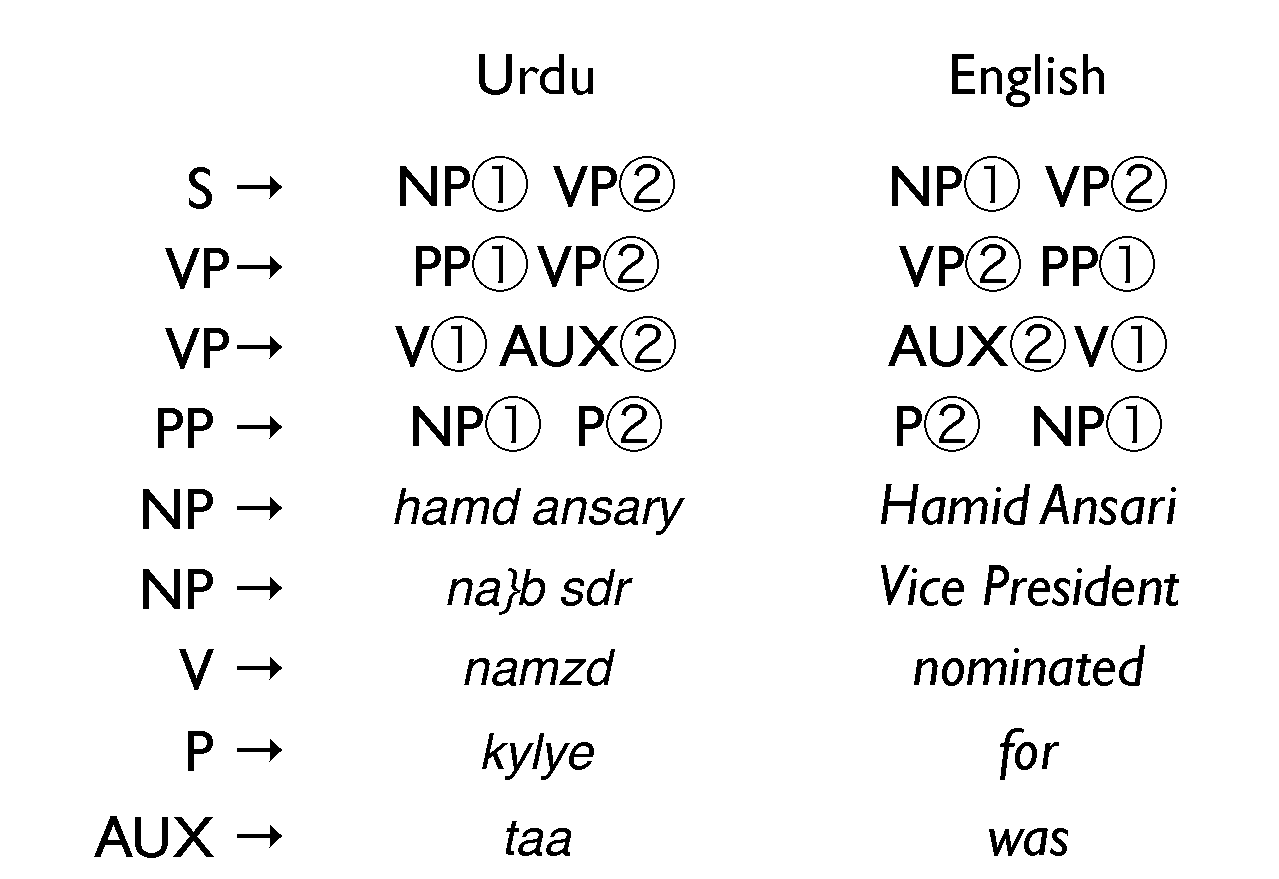
\includegraphics[width=.6\linewidth]{SCFGs/example-scfg}
\end{center}
\caption{A toy example that illustrates a SCFG that can translate (romanized) Urdu into English for one sentence.    }\label{fig:toy-scfg} 
\end{figure}



\begin{figure}
\begin{tabular}{lll}
\multicolumn{3}{>{\columncolor[rgb]{0.95,0.95,0.75}}c}{The input is an Urdu sentence which is initially unanalyzed.}\\
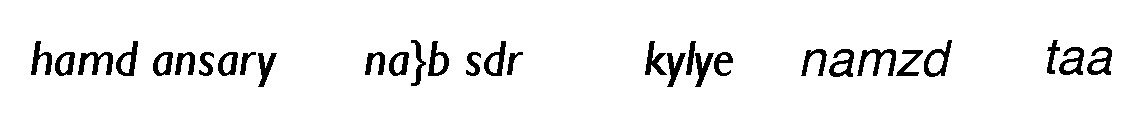
\includegraphics[width=.45\linewidth]{SCFGs/urdu-input} &  & 
\\ \hline
\multicolumn{3}{>{\columncolor[rgb]{0.95,0.95,0.75}}c}{Here all of the terminal symbols receive non-terminal labels.  The English words are in Urdu order.}\\
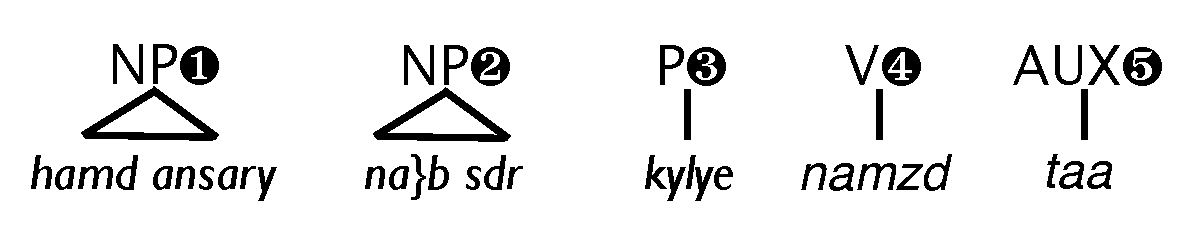
\includegraphics[width=.45\linewidth]{SCFGs/urdu-step0} & &
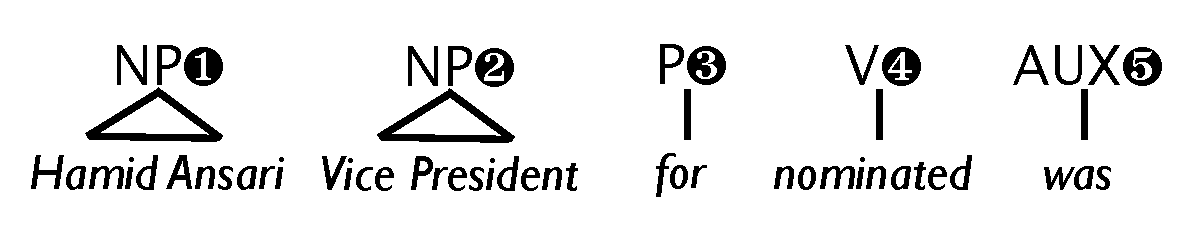
\includegraphics[width=.45\linewidth]{SCFGs/english-step0} \\ \hline
\multicolumn{3}{>{\columncolor[rgb]{0.95,0.95,0.75}}c}{The PP rule reorders the Urdu postpositional phrase to be a prepositional phrase on the English side.}\\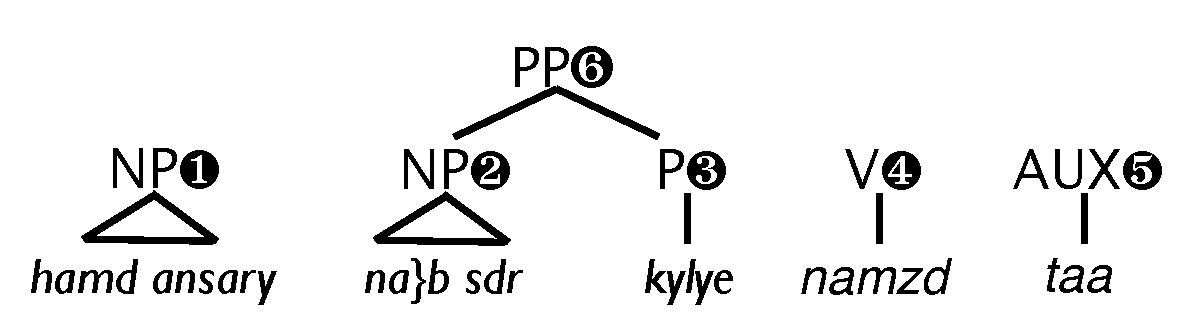
\includegraphics[width=.45\linewidth]{SCFGs/urdu-step1} & &
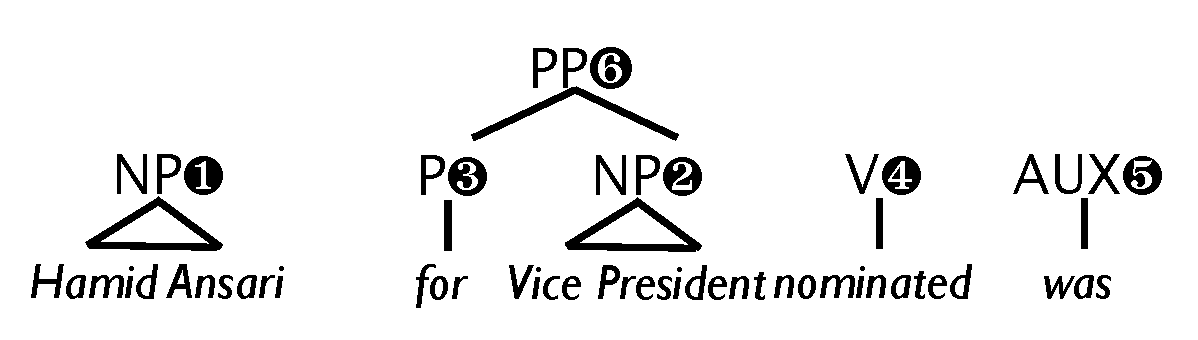
\includegraphics[width=.45\linewidth]{SCFGs/english-step1} \\ \hline\multicolumn{3}{>{\columncolor[rgb]{0.95,0.95,0.75}}c}{The English auxiliary verb and main verb get reordered with the application of the VP rule.}\\
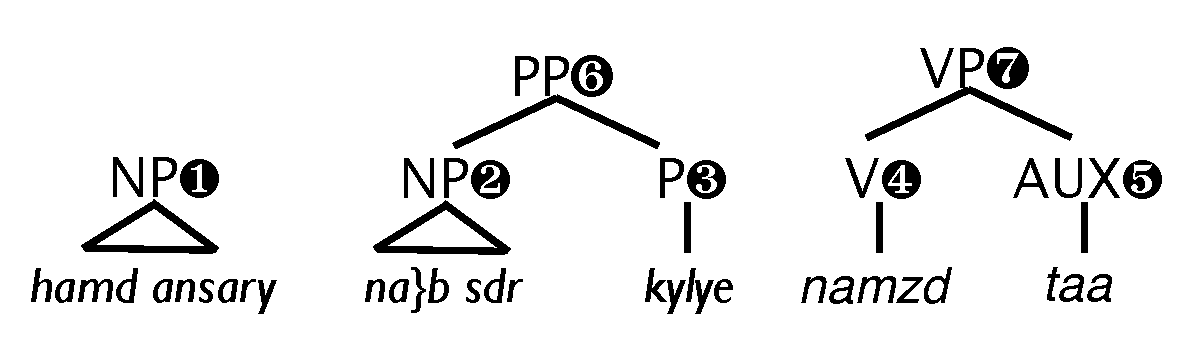
\includegraphics[width=.45\linewidth]{SCFGs/urdu-step2} & &
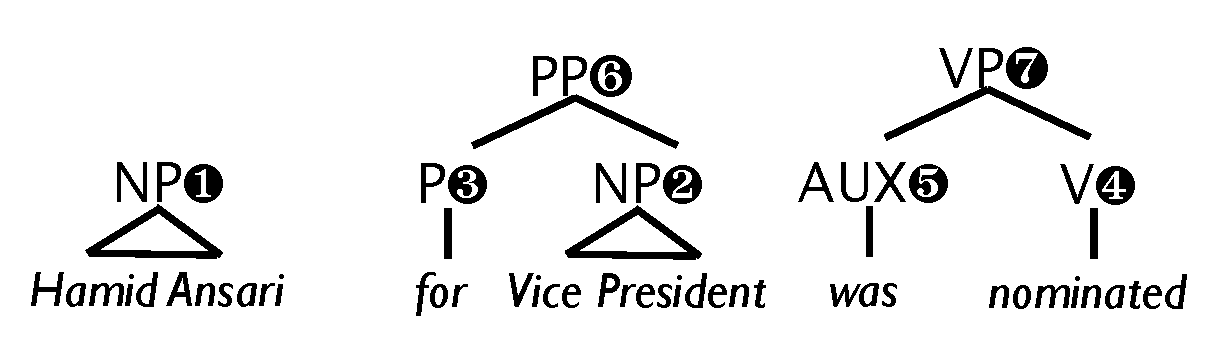
\includegraphics[width=.45\linewidth]{SCFGs/english-step2} \\ \hline 
\multicolumn{3}{>{\columncolor[rgb]{0.95,0.95,0.75}}c}{This VP rule moves the English verb from the Urdu verb-final position to its correct place before the PP.}\\
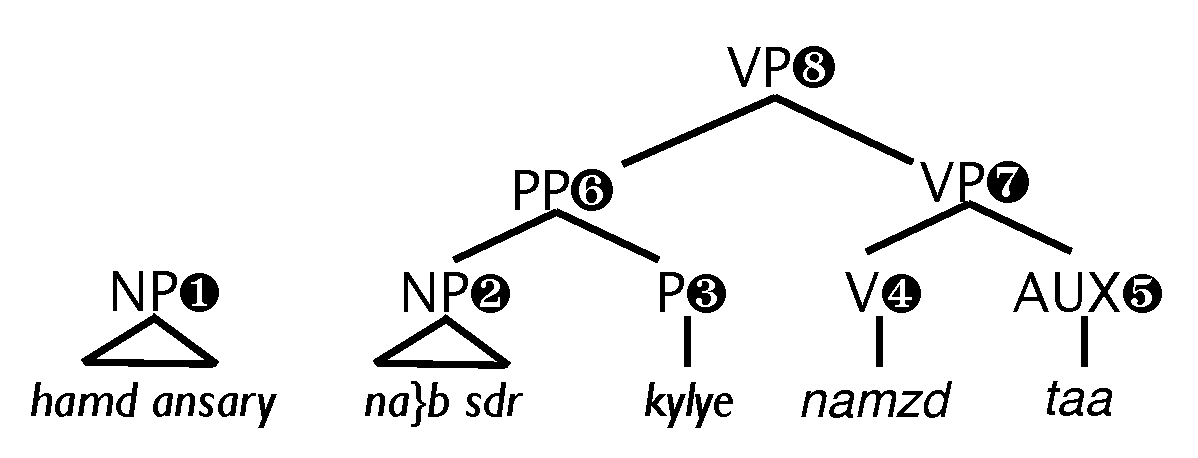
\includegraphics[width=.45\linewidth]{SCFGs/urdu-step3} &  & 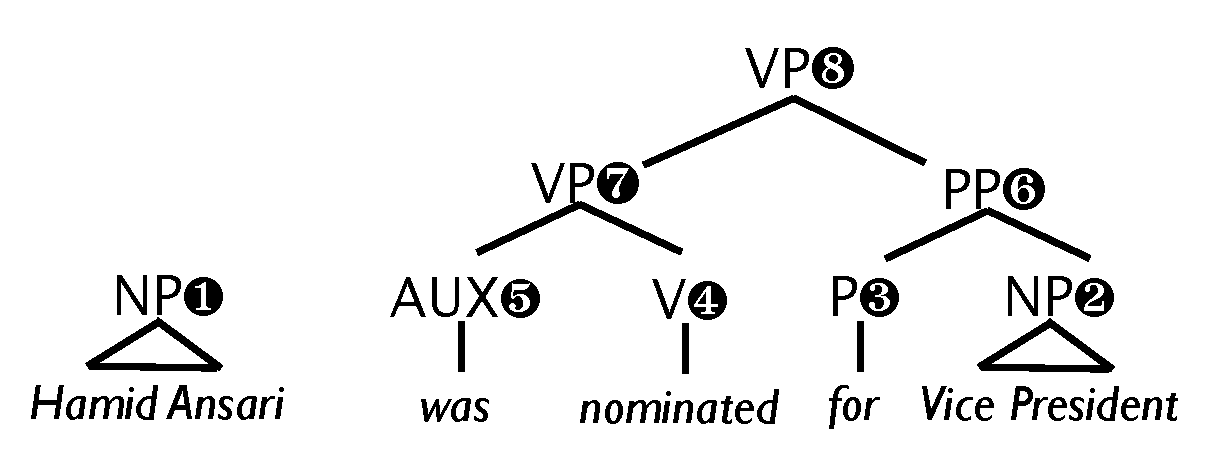
\includegraphics[width=.45\linewidth]{SCFGs/english-step3} \\ \hline
\multicolumn{3}{>{\columncolor[rgb]{0.95,0.95,0.75}}c}{Applying the S rule, means that we have a complete translation of the Urdu sentence.}\\
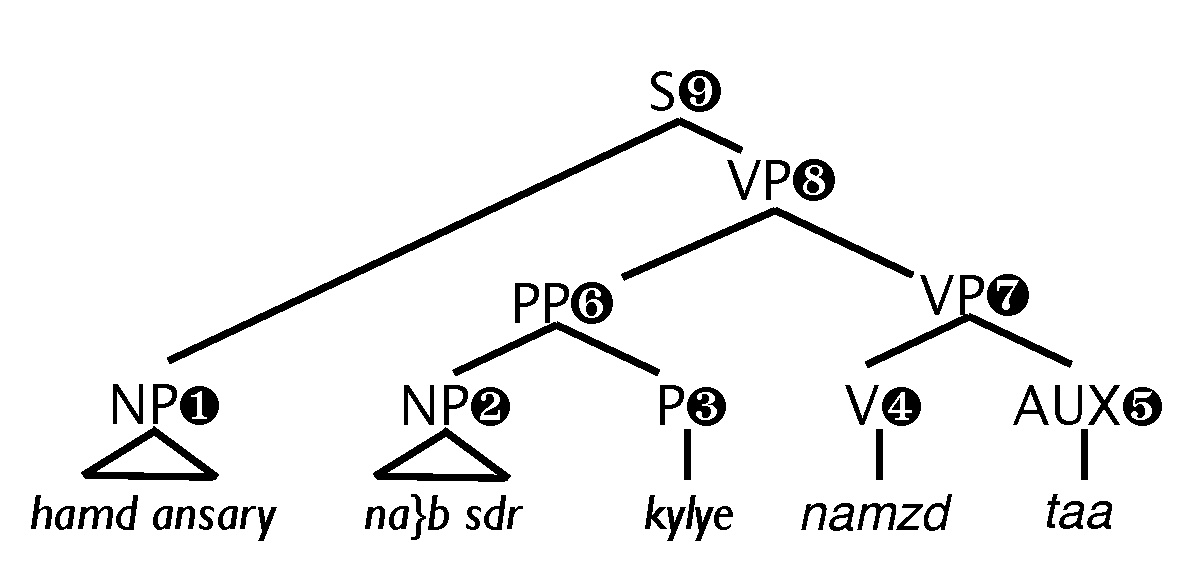
\includegraphics[width=.45\linewidth]{SCFGs/urdu-step4} &  & 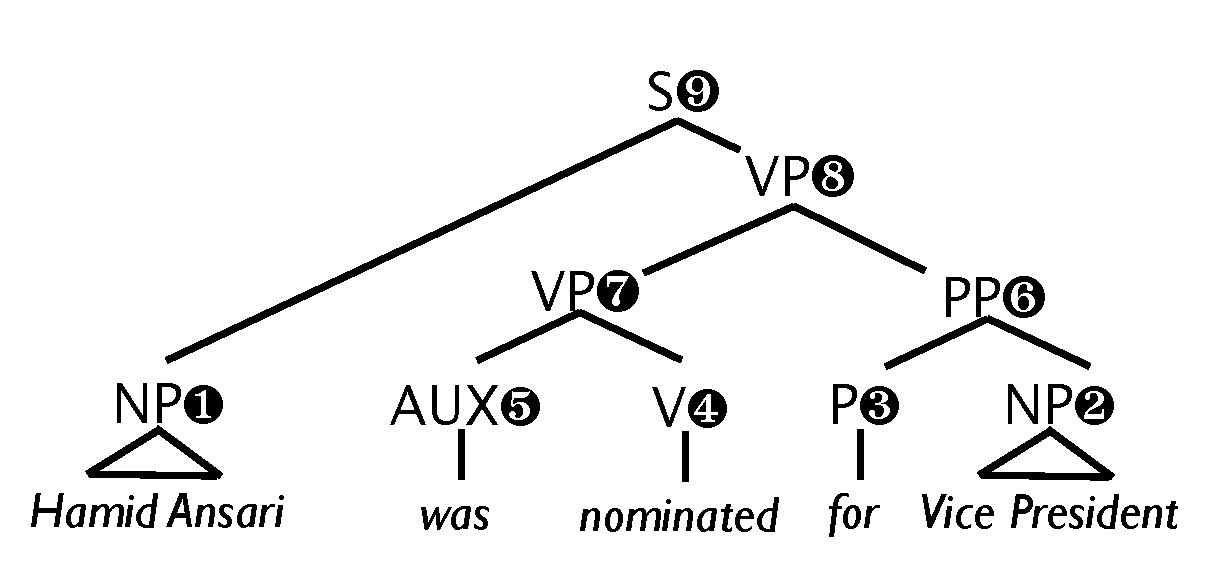
\includegraphics[width=.45\linewidth]{SCFGs/english-step4} 
\end{tabular}
\caption{Using SCFGs as the underlying formalism means that the process of translation is one of parsing.  This shows how an English sentence can be generated by parsing the Urdu sentence using the rules given in Figure \ref{fig:toy-scfg}}\label{fig:toy-scfg-parse} 
\end{figure}






% of the form that I propose to learn using non-parametric Bayesian models.

The generative story is as follows. 
In the beginning was the grammar, in which we allow  two types of rules: {\emph non-terminal} and {\emph terminal} expansions. 
The former rewrites a non-terminal symbol as a string of two or three non-terminals along with an alignment $\mathbf{a}$, specifying the corresponding ordering of the child trees in the source and target language. 
Terminal expansion rewrite a non-terminal as a pair of terminal n-grams, where either but not both may be empty. 
Given a grammar, each sentence is generated as follows, starting with the distinguished root non-terminal, $S$. 
Rewrite each frontier non-terminal, $c$, using a rule chosen from our grammar expanding $c$. 
Repeat until there are no remaining frontier non-terminals. 
The sentences in both languages can then be read off the leaves, using the rules' alignments to find the right ordering. 

\begin{figure}[t]
  \centering
  \subfigure{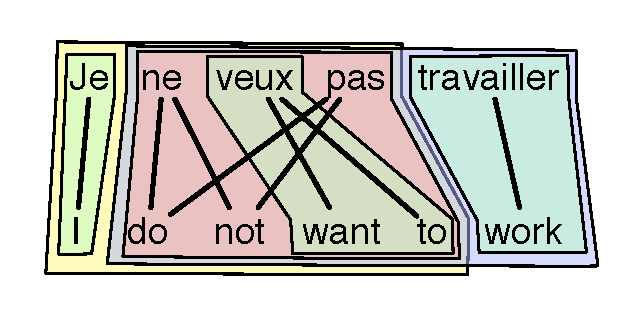
\includegraphics[scale=0.7]{intro_slides/PhraseExtraction1.pdf}}
  \subfigure{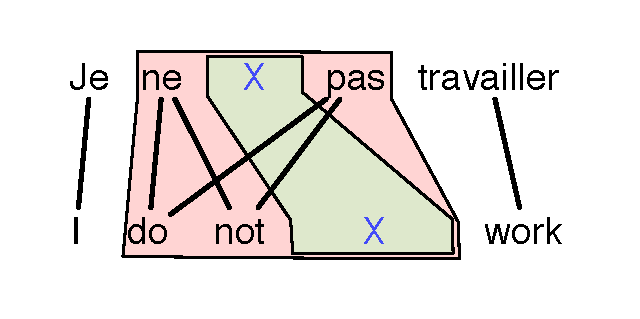
\includegraphics[scale=0.7]{intro_slides/HieroExtraction2.pdf}}
\caption{Extracting translation rules from aligned sentences. All the phrases obtained using the standard phrase extraction heuristics are depicted in the left figure, these are: $\langle$ Je, I $\rangle$, $\langle$ veux, want to $\rangle$, $\langle$ travailler, work $\rangle$, $\langle$ ne veux pas, do not want to $\rangle$, $\langle$ ne veux pas travailler, do not want to work $\rangle$, $\langle$ Je ne veux pas, I do not want to $\rangle$, $\langle$ Je ne veux pas travailler, I do not want to work $\rangle$. On the right is shown how a discontiguous SCFG rule is created by generalising a phrase embedded in another phrase, the extracted rule is: X $\rightarrow$ $\langle$ ne X$_1$ pas, do not X$_1$ $\rangle$.}
\label{fig:intro_rule_extraction}
\end{figure}

The process for extracting SCFG rules is based on that used to extract translation phrases in phrase based translation systems. 
The phrase based approach \cite{koehn03} uses heuristics to extract phrase translation pairs from a word-aligned corpus. 
The phrase extraction heuristic is illustrated in Figure \ref{fig:intro_rule_extraction}. 
This heuristic extracts all phrases whose words are either not aligned, or aligned with only other words in the same phrase. 
The phrase translation probabilities are then calculated using a maximum likelihood estimation. 

The Hiero \cite{chiang07hierarchical} SCFG extraction heuristic starts from a grammar consisting of the set of contiguous phrases, wherever a phrase is wholly embedded within another a new rule is add with the embedded phrase replace by the non-terminal X. 
This process continues until all possible rules have been extracted, subject to the constraints that every rule must contain a terminal on the source side, a rule may only contain two non-terminals on its right side and that those non-terminals may not be adjacent.
The left example in Figure \ref{fig:intro_rule_extraction} depicts this rule generalisation process. 
